\section{Heuristics}


\begin{frame}{Plan}

    \vspace{-0.5cm}
    \begin{table}[]
    \renewcommand{\arraystretch}{1.5}
        \begin{tabular}{ll}
          \labelitem Simple linear model & $Y_i = \beta_0 + \sum_{s = 1}^S \beta_s X_i(\tau_s) + \epsilon_i$\\
          \labelitem Gaussian Process Regressors &  $X_i \sim \mathcal{GP}(0, \sigma)$\\
        \end{tabular}
    \end{table}

    \vspace{0.5cm}
    \begin{table}[]
    \renewcommand{\arraystretch}{1.5}
        \begin{tabular}{ll}
            \blue{Task:} & Think of how to identify/estimate $\tau_s$ for different $\sigma$\\
            \grey{Kernels:} & White, Brownian Motion, Matern, RBF\\
            \yellow{First insight:} & Investigate object $\expectation{Y_i X_i(t)}$
        \end{tabular}
    \end{table}

\end{frame}


\begin{frame}{Building Intuition}

    What is the connection between the kernel and a sample trajectory?\\[2em]

    $\implies$ Visualization

\end{frame}


\begin{frame}{General Representation}

    \vspace{-0.5cm}
    \begin{align*}
    \label{eq:1}
    f_{XY}(t) &\stackrel{def}{=} \expectation{Y_i X_i(t)}\\
              &= \expectation{\left(\beta_0 + \sum_{s = 1}^S \beta_s X_i(\tau_s) + \epsilon_i\right) X_i(t)}\\
              &= \sum_{s = 1}^S \beta_s \, \expectation{X_i(\tau_s) X_i(t)}\\
              &= \sum_{s = 1}^S \beta_s \, \sigma(t, \tau_s)
    \end{align*}

\end{frame}


\begin{frame}{White Kernel}

\vspace{-1.2cm}
\begin{centering}
\begin{tikzpicture}

    \draw node at (8.35, 4) {$\sigma(s, t) = \indicator{s = t}$};
    \draw node at (9, 3) {$f_{XY}(t) = \sum_{s = 1}^S \beta_s \, \sigma(t, \tau_s)$};
    \draw node at (9.65, 2.2) {$= \sum_{s = 1}^S \beta_s \, \indicator{t = \tau_s}$};

    \draw[line width=0.25mm, ->] (0, -2.5) -- (0, 3.5) node [left] {$f_{XY}$};
    \draw[line width=0.25mm, ->] (-0.5, 0) -- (11, 0) node [below] {$t$};

    \draw (10, -0.2) -- (10, 0.2) node [below=0.4cm] {$1$};
    \draw node at (-0.2, -0.2) {$0$};

    \draw[line width=0.25mm] (2.5, -0.2) -- (2.5, 0) node [below=0.2cm] {$\tau_1$};
    \draw[line width=0.25mm] (5, -0.2) -- (5, 0) node [below=0.2cm] {$\tau_2$};
    \draw[line width=0.25mm] (7.5, 0) -- (7.5, 0.2) node [above] {$\tau_3$};

    \draw[line width=0.25mm, color=bonnblue] (0.02, 0.03) -- (9.98, 0.03) {};

    \draw[line width=0.25mm, color=bonnblue] (2.5, 0.03) -- (2.5, 1) node [left] {$\beta_1$};
    \draw[line width=0.25mm, color=bonnblue] (5, 0) -- (5, 3) node [left] {$\beta_2$};
    \draw[line width=0.25mm, color=bonnblue] (7.5, -0.03) -- (7.5, -2) node [left] {$\beta_3$};

    \draw[line width=0.2mm, color=bonngrey, dashed] (1.9, 1) -- (0, 1) node [left] {$1$};
    \draw[line width=0.2mm, color=bonngrey, dashed] (4.4, 3) -- (0, 3) node [left] {$3$};
    \draw[line width=0.2mm, color=bonngrey, dashed] (6.9, -2) -- (0, -2) node [left] {$-2$};

\end{tikzpicture}
\end{centering}
    
\end{frame}


\begin{frame}{Brownian Motion}

\vspace{-1.2cm}
\begin{centering}
\begin{tikzpicture}

    \draw node at (8.35, 4) {$\sigma(s, t) = \min\{s, t\}$};
    \draw node at (9, 3) {$f_{XY}(t) = \sum_{s = 1}^S \beta_s \, \sigma(t, \tau_s)$};
    \draw node at (9.65, 2.2) {$= \sum_{s = 1}^S \beta_s \, \min\{t, \tau_s\}$};

    \draw[line width=0.25mm, ->] (0, -2.5) -- (0, 3.5) node [left] {$f_{XY}$};
    \draw[line width=0.25mm, ->] (-0.5, 0) -- (11, 0) node [below] {$t$};

    \draw (10, -0.2) -- (10, 0.2) node [below=0.4cm] {$1$};
    \draw node at (-0.2, -0.2) {$0$};

    \draw[line width=0.25mm] (2.5, -0.2) -- (2.5, 0) node [below=0.2cm] {$\tau_1$};
    \draw[line width=0.25mm] (5, -0.2) -- (5, 0) node [below=0.2cm] {$\tau_2$};
    \draw[line width=0.25mm] (7.5, -0.2) -- (7.5, 0) node [below=0.2cm] {$\tau_3$};

    \draw[line width=0.25mm, dashed, color=bonngrey] (2.5, 0) -- (2.5, 1);
    \draw[line width=0.25mm, dashed, color=bonngrey] (5, 0) -- (5, 1.5);
    \draw[line width=0.25mm, dashed, color=bonngrey] (7.5,0) -- (7.5, 0.5);

    \draw[line width=0.25mm, color=bonnblue] (0.02, 0.03) -- (2.5, 1);
    \draw[line width=0.25mm, color=bonnblue] (2.5, 1) -- (5, 1.5);
    \draw[line width=0.25mm, color=bonnblue] (5, 1.5) -- (7.5, 0.5);
    \draw[line width=0.25mm, color=bonnblue] (7.5, 0.5) -- (10, 0.5);

\end{tikzpicture}
\end{centering}
    
\end{frame}


\begin{frame}

    \begin{center}
        \includegraphics[width=0.95\textwidth]{../../bld/figures/cross-covariance.png}
    \end{center}

\end{frame}


\begin{frame}{How do we find $\tau$?}

\begin{centering}
\begin{tikzpicture}[scale=2.5]
    \draw[line width=0.25mm, ->] (0, -0.3) -- (0, 2.2);
    \draw[line width=0.25mm, ->] (-0.3, 0) -- (4, 0);

    \draw (0, 0) .. controls (1, 1) and (1.5, 1.5) .. (0.2*8, 2);
    \draw (0.2*8, 2) .. controls (2, 1) and (3, 0.75) .. (4, 0.5);

    \draw[line width=0.2mm, dashed, color=bonngrey] (0.2*8, 0.07) -- (0.2*8, 2);
    \draw node at (0.2*8, -0.15) {\small $\tau$};

    \foreach \x in {1,...,19}
        \draw[thin] (0.2*\x, 0.07) -- (0.2*\x, -0.07);

    \draw[thin, dashed, color=bonnblue] (0.2*13, 0.07) -- (0.2*13, 0.97);
    \draw[thin, dashed, color=bonnblue] (0.2*14, 0.07) -- (0.2*14, 0.86);
    \draw[thin, dashed, color=bonnblue] (0.2*15, 0.07) -- (0.2*15, 0.79);
    \draw node at (0.2*14, -0.15) {$t$};

    \draw[thin, dashed, color=bonnblue] (0.2*13, 0.97) -- (0, 0.97) node [left] {\tiny
        $f(t - \delta)$};
    \draw[thin, dashed, color=bonnblue] (0.2*14, 0.86) -- (-0.45, 0.86) node [left] {\tiny
        $f(t)$};
    \draw[thin, dashed, color=bonnblue] (0.2*15, 0.79) -- (0, 0.79) node [left] {\tiny
        $f(t + \delta)$};

    \draw node at (3, 2.2) {\blue{$|\,f(t) - \frac{1}{2} (f(t - \delta) + f(t + \delta))| \approx
        0$}};

    \draw[thin, dashed, color=bonngrey] (0.2*7, 0.07) -- (0.2*7, 1.57);
    \draw[line width=0.2mm, dashed, color=bonngrey] (0.2*8, 0) -- (0.2*8, 2);
    \draw[thin, dashed, color=bonngrey] (0.2*9, 0.07) -- (0.2*9, 1.63);
    
    \draw[thin, dashed, color=bonngrey] (0.2*7, 1.57) -- (0, 1.57) node [left] {\tiny
        $f(\tau - \delta)$};
    \draw[thin, dashed, color=bonngrey] (0.2*8, 2)   -- (0, 2) node [left] {\tiny
        $f(\tau)$};
    \draw[thin, dashed, color=bonngrey] (0.2*9, 1.63)-- (0, 1.63) node [left] {\tiny
        $f(\tau + \delta)$};

    \draw node at (3.2, 1.8) {\grey{$|\,f(\tau) - \frac{1}{2} (f(\tau - \delta) + f(\tau +
    \delta))| \gg 0$}};


\end{tikzpicture}
\end{centering}

\end{frame}


\begin{frame}{How do we find $\tau$?}

\begin{centering}
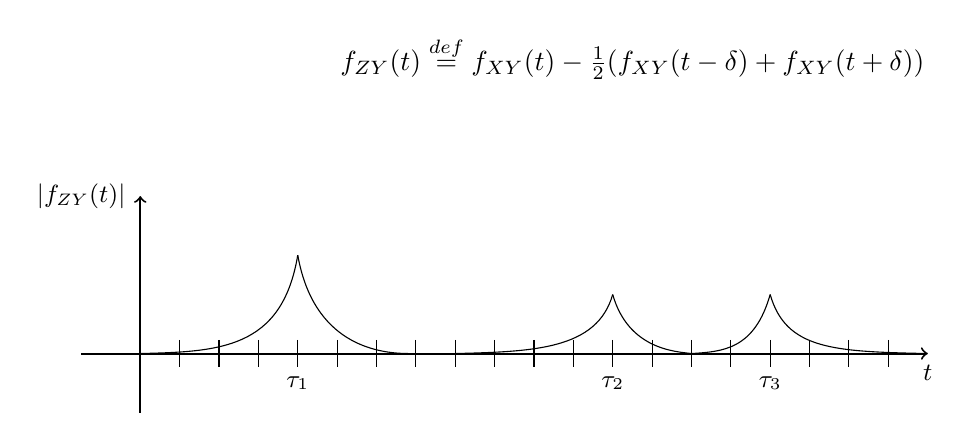
\begin{tikzpicture}[scale=2.5]
    \draw[line width=0.25mm, ->] (0, -0.3) -- (0, 0.8);
    \draw[line width=0.25mm, ->] (-0.3, 0) -- (4, 0);

    \draw (0, 0) .. controls (0.05*8, 0.01) and (0.09*8, 0.02) .. (0.1*8, 0.5);
    \draw (0.1*8, 0.5) .. controls (0.11*8, 0.05) and (0.15*8, 0.001) .. (0.17*8, 0);

    \draw (0.2*8, 0) .. controls (0.25*8, 0.01) and (0.29*8, 0.02) .. (0.3*8, 0.3);
    \draw (0.3*8, 0.3) .. controls (0.31*8, 0.02) and (0.34*8, 0.01) .. (0.35*8, 0);

    \draw (0.35*8, 0) .. controls (0.37*8, 0.01) and (0.39*8, 0.02) .. (0.4*8, 0.3);
    \draw (0.4*8, 0.3) .. controls (0.41*8, 0.02) and (0.44*8, 0.01) .. (0.5*8, 0);

    \draw node at (0.1*8, -0.15) {\small $\tau_1$};
    \draw node at (0.3*8, -0.15) {\small $\tau_2$};
    \draw node at (0.4*8, -0.15) {\small $\tau_3$};
    \draw node at (-0.3, 0.8) {\small $|f_{ZY}(t)|$};
    \draw node at (4, -0.1) {\small $t$};

    \foreach \x in {1,...,19}
        \draw[thin] (0.2*\x, 0.07) -- (0.2*\x, -0.07);

        \draw node at (2.5, 1.5) {$f_{ZY}(t) \stackrel{def}{=} f_{XY}(t) -
            \frac{1}{2}(f_{XY}(t - \delta) + f_{XY}(t + \delta))$};

\end{tikzpicture}
\end{centering}

\end{frame}



% \begin{frame}{Finite Difference and Differentiability}
%     \vspace{-1cm}
%     Let $h: [0, 1] \to \mathbb{R}$.
% 
%     \vspace{0.25cm}
%     \blue{Definition.}\\
%         \quad $h$ is differentiable at $t \in (0, 1)$ if
%         $\lim_{\delta \to 0} (h(t + \delta) - h(t - \delta)) / \delta$ exists.
% 
%     \vspace{0.5cm}
%     \blue{Definition.}\\
%         \quad $C = C(t, \delta; h) = h(t + \delta) - h(t - \delta)$ is the (first-order)
%         centered difference of $h$.\\
%         \quad For small $\delta$, $h'(t)$ is approximated by $C / \delta$.
% 
%     \vspace{0.5cm}
%     \blue{Second derivative.}\\
%         \quad Applying the first-order centered difference twice yields the second-order\\
%         \quad difference $C^2 = C^2(t, \delta; h) = h(t + \delta) + h(t - \delta) -
%         2h(t)$. For small $\delta$, $h''(t)$ is\\ \quad approximated by $C^2 / \delta$.
% 
% \end{frame}


% \begin{frame}{Connecting Ideas}
% 
%     \begin{itemize}
%     \setlength\itemsep{1.5em}
%         \item[\labelitem] $f_{XY}(t) - \frac{1}{2}\left(f_{XY}(t + \delta) + f_{XY}(t -
%             \delta)\right) $ \pause
%         \item[\labelitem] $C^2(t, \delta; f_{XY}) = \left(f_{XY}(t + \delta) + f_{XY}(t
%             - \delta)\right) - 2 f_{XY}(t)$ \pause
%         \item[\labelitem] $\implies C^2(t, \delta; f_{XY}) = - 2 \Big[ f_{XY}(t) -
%                 \frac{1}{2} \left(f_{XY}(t + \delta) + f_{XY}(t - \delta)\right) \Big]$
%     \end{itemize}
% 
% \end{frame}


\begin{frame}{Estimation?}
    \begin{itemize}
    \setlength\itemsep{1.5em}
        \item[\labelitem] $Z_{\delta, i}(t) := X_i(t) - \left(X_i(t + \delta) + X_i(t -
            \delta)\right) / 2$
        \item[\labelitem] $\implies \expectation{Z_{\delta, i}(t) Y_i} = f_{XY}(t) -
            \frac{1}{2}\left(f_{XY}(t + \delta) + f_{XY}(t - \delta)\right) = f_{ZY}(t)$
        \item[\labelitem] Estimate by: $\,\, \hat{f}_{ZY}(t) = n^{-1}\sum_{i=1}^n
            Z_{\delta, i}(t) Y_i$
        \item[\labelitem] But what about $\delta$? $\implies$ Visualization
    \end{itemize}
\end{frame}
